\documentclass[journal,onecolumn]{IEEEtran}

\usepackage{graphicx}
\usepackage{bbm}
\usepackage{amsfonts,amssymb,amsmath,amsthm}
\usepackage{type1cm,eso-pic,color}
\usepackage{mathrsfs} 
\usepackage{mathpazo}
\usepackage[scaled=.95]{helvet}
\usepackage{courier}
\usepackage{xspace}
\usepackage{etoolbox}
\usepackage[shortlabels]{enumitem}
\usepackage{multirow}
\usepackage{dsfont}
\usepackage{hhline}
\usepackage{graphicx}

\usepackage{xr}
\externaldocument[I-]{../BoundEffRed2}


\def\matlab{{\sc Matlab\ }}
\def\octave{{\sc Octave}}
\renewcommand{\Re}{\operatorname{Re}}
\renewcommand{\Im}{\operatorname{Im}}


%\def\foorp{{\hfill$\spadesuit$}}
\def\foorp{{\hfill$\square$}}
\def\ds{{\displaystyle}}
\def\inv{{^{-1}}}
\def\HH{{\mathbb H}}
\def\MM{{\mathbb M}}
\def\tMM{\tilde{\mathbb M}}
\def\RR{{\mathbb R}}
\def\SS{{\mathbb S}}
\def\PP{{\mathbb P}}
\def\EE{{\mathbb E}}
\def\Pr#1{{\PP\!\left\{#1\right\}}}
\def\Ex#1{{\EE\left\{#1\right\}}}
\def\var#1{{\hbox{Var}\left\{#1\right\}}}
\def\QQ{\mathbb Q}
\def\CC{\mathbb C}
\def\ZZ{\mathbb Z}
\def\NN{\mathbb N}
\def\Id{{\mathbbm 1}}
\def\cN{\mathcal N}
\def\dd#1{\mathrm{d}#1}

\def\tX{\tilde{X}}

\def\ii{\mathrm{i}}

\def\1{\mathds{1}}

%\def\o{\overline}
\def\la{\langle}
\def\ra{\rangle}

\def\ch{{\rm ch}}
\def\sh{{\rm sh}}


\def\rf#1{(\ref{#1})}
\def\be{\begin{equation}}
\def\beq#1{\begin{equation}\label{#1}}
\def\ee{\end{equation}}
\def\bea{\begin{eqnarray}}
\def\beqa#1{\begin{eqnarray}\label{#1}}
\def\eea{\end{eqnarray}}
\def\ba{\begin{array}}
\def\ea{\end{array}}


\DeclareMathAlphabet{\mathpzc}{OT1}{pzc}{m}{it}

\def\defeq{\overset{\Delta}{=}}

\def\eg{e.g.\@}
\def\ie{i.e.\@}
\def\etal{\textit{et al.}}


\def\cA{{\mathcal A}}
\def\cB{{\mathcal B}}
\def\cC{{\mathcal C}}
\def\ccC{{\mathscr C}}
\def\cCN{{\mathcal {C\!N}}}
\def\tcC{\tilde{\mathcal C}}
\def\cD{{\mathcal D}}
\def\ccD{{\mathscr D}}
\def\cE{{\mathcal E}}
\def\cF{{\mathcal F}}
\def\ccF{{\mathscr F}}
\def\cG{{\mathcal G}}
\def\ccG{{\mathcal G}}
\def\ocF{\overline{\mathcal F}}
\def\cH{{\mathcal H}}
\def\ccH{{\mathscr H}}
\def\cJ{{\mathcal J}}
\def\ck{{\mathcal k}}
\def\cK{{\mathcal K}}
\def\cL{{\mathcal L}}
\def\ccL{{\mathscr L}}
\def\cM{{\mathcal M}}
\def\ccM{{\mathscr M}}
\def\cN{{\mathcal N}}
\def\cP{{\mathcal P}}
\def\cQ{{\mathcal Q}}
\def\ccQ{{\mathscr Q}}
\def\cR{{\mathcal R}}
\def\ccR{{\mathscr R}}
\def\cS{{\mathcal S}}
\def\ccS{{\mathscr S}}
\def\cT{{\mathcal T}}
\def\ccT{{\mathscr T}}
\def\cO{{\mathcal O}}
\def\cU{{\mathcal U}}
\def\tcU{\widetilde{\mathcal U}}
\def\cV{{\mathcal V}}
\def\tcV{\widetilde{\mathcal V}}
\def\cW{{\mathcal W}}
\def\tcW{\widetilde{\mathcal W}}
\def\cl{{\mathpzc l}}
\def\cs{{\mathpzc s}}




\def\la{{\langle}}
\def\ra{{\rangle}}
\def\qed{\hskip 6pt\vrule height6pt width5pt depth1pt}
\def\R{\RR}
\def\Z{\ZZ}
\def\sgn{\hbox{sgn}}
\def\Lone{L^1(\RR )}
\def\Ltwo{L^2(\RR )}
\def\Linf{L^\infty(\RR )}
\def\Lba{L^2(\RR\times\RR_+^* ,a^{-1}dadb)}
\def\Htwo{H^2(\RR )}
\def\lone{\ell^1(\ZZ )}
\def\ltwo{\ell^2(\ZZ )}
\def\gets{$<\!\!\! -\,$}
%\def\Id{{\bf 1}}
\def\bds{_{-\infty}^\infty}
\def\supp{\hbox{supp}}
\def\mod{{\mathrm {mod}}}
\def\modN{[\hbox{\footnotesize mod }N]}

% bold
\def\bpsi{\boldsymbol{\psi}}
\def\bPsi{\boldsymbol{\Psi}}
\def\balpha{\boldsymbol{\alpha}}
\def\bbeta{\boldsymbol{\beta}}
\def\bDelta{\boldsymbol{\Delta}}
\def\bzero{\boldsymbol{0}}
\def\blambda{\boldsymbol{\lambda}}
\def\bLambda{\boldsymbol{\Lambda}}
\def\bSigma{\boldsymbol{\Sigma}}
\def\bepsilon{\boldsymbol{\epsilon}}
\def\bgamma{\boldsymbol{\gamma}}
\def\bGamma{\boldsymbol{\Gamma}}
\def\bmu{\boldsymbol{\mu}}
\def\bnabla{\boldsymbol{\nabla}}
\def\bphi{\boldsymbol{\varphi}}
\def\bPsi{\boldsymbol{\Psi}}
\def\brho{\boldsymbol{\rho}}
\def\btheta{\boldsymbol{\theta}}
\def\bTheta{\boldsymbol{\Theta}}
\def\btau{\boldsymbol{\tau}}
\def\bxi{\boldsymbol{\xi}}
\def\bnu{\boldsymbol{\nu}}
\def\bOmega{\boldsymbol{\Omega}}

\def\ba{{\mathbf a}}
\def\bA{{\mathbf A}}
\def\bb{{\mathbf b}}
\def\bB{{\mathbf B}}
\def\bC{{\mathbf C}}
\def\bD{{\mathbf D}}
\def\be{{\mathbf e}}
\def\bE{{\mathbf E}}
\def\bff{{\mathbf f}}
\def\bF{{\mathbf F}}
\def\bg{{\mathbf g}}
\def\bG{{\mathbf G}}
\def\bh{{\mathbf h}}
\def\bH{{\mathbf H}}
\def\bI{{\mathbf I}}
\def\bJ{{\mathbf J}}
\def\bK{{\mathbf K}}
\def\bL{{\mathbf L}}
\def\bm{{\mathbf m}}
\def\bM{{\mathbf M}}
\def\bN{{\mathbf N}}
\def\bo{{\mathbf o}}
\def\bO{{\mathbf O}}
\def\bP{{\mathbf P}}
\def\bq{{\mathbf q}}
\def\bQ{{\mathbf Q}}
\def\br{{\mathbf r}}
\def\bR{{\mathbf R}}
\def\bs{{\mathbf s}}
\def\bS{{\mathbf S}}
\def\bt{{\mathbf t}}
\def\bT{{\mathbf T}}
\def\bu{{\mathbf u}}
\def\bU{{\mathbf U}}
\def\bv{{\mathbf v}}
\def\bV{{\mathbf V}}
\def\bw{{\mathbf w}}
\def\bW{{\mathbf W}}
\def\bx{{\mathbf x}}
\def\bX{{\mathbf X}}
\def\by{{\mathbf y}}
\def\bY{{\mathbf Y}}
\def\bZ{{\mathbf Z}}
\def\bz{{\mathbf z}}

% overline
\def\ox{\overline{x}}
\def\oy{\overline{y}}
\def\oz{\overline{z}}

% tilde
\def\tb{{\tilde{b}}}
\def\te{{\tilde{e}}}
\def\tf{{\tilde{f}}}
\def\tg{{\tilde{g}}}
\def\th{{\tilde{h}}}
\def\tk{{\tilde{k}}}
%\def\tt{{\tilde{t}}}
\def\tp{{\tilde{p}}}
\def\tu{{\tilde{u}}}
\def\tv{{\tilde{v}}}
\def\tx{{\tilde{x}}}
\def\ty{{\tilde{y}}}
\def\tz{{\tilde{z}}}
\def\tp{{\tilde{p}}}
\def\tq{{\tilde{q}}}

\def\tgamma{{\tilde\gamma}}
\def\tGamma{{\tilde\Gamma}}
\def\tsigma{{\tilde\sigma}}
\def\tSigma{{\tilde\Sigma}}
\def\tpi{{\tilde\pi}}
\def\tpsi{{\tilde\psi}}
\def\trho{{\tilde\rho}}
\def\tX{{\tilde{X}}}
\def\tY{{\tilde{Y}}}
\def\S{{\tilde{S}}}
\def\T{{\tilde{T}}}

% hat
\def\hb{{\hat b}}
\def\he{{\hat e}}
\def\hh{{\hat h}}
\def\hk{{\hat k}}
\def\hp{{\hat p}}
% \def\ht{{\hat t}}
\def\hu{{\hat u}}
\def\hv{{\hat v}}
\def\hw{{\hat w}}
\def\hx{{\hat x}}
\def\hy{{\hat y}}
\def\hz{{\hat z}}
\def\hLambda{{\hat \Lambda}}
\def\hDelta{{\hat \delta}}
\def\hlambda{{\hat \lambda}}
\def\hdelta{{\hat \delta}}
\def\halpha{{\hat \alpha}}
\def\hbeta{{\hat \beta}}
\def\htheta{{\hat \theta}}
\def\hsigma{{\hat \sigma}}


% vectors (underline)
\def\a{{\underline{a}}}
\def\e{{\underline{e}}}
\def\h{{\underline{h}}}
\def\k{{\underline{k}}}
\def\m{{\underline{m}}}
\def\t{{\underline{t}}}
\def\u{{\underline{u}}}
\def\w{{\underline{w}}}
\def\x{{\underline{x}}}
\def\y{{\underline{y}}}
\def\z{{\underline{z}}}

\def\X{{\underline{X}}}
\def\Y{{\underline{Y}}}
\def\S{{\underline{S}}}
\def\T{{\underline{T}}}

\def\Om{{\underline{\Omega}}}

\def\ual{{\underline\alpha}}
\def\ubet{{\underline\beta}}
%
% Matrices
\def\A{{\underline{\underline{A}}}}
\def\RX{{\underline{\underline{R}}_X}}

%
% Algebraic quantities
\def\rg#1{{\hbox{rg}\left(#1\right)}}

\def\fs{f_{\mathsf s}}


\title{An Efficient Forecasting Approach for the Real-Time Reduction of Boundary Effects\\ in Time-Frequency Representations:\\ Part II}

\author{Adrien~Meynard, %~\IEEEmembership{Member,~IEEE,}
        Hau-Tieng~Wu
\thanks{A. Meynard and H.-T. Wu are with the Department
of Mathematics, Duke University, Durham,
NC, 27708 USA e-mail: adrien.meynard@duke.edu}}

\newtheorem{remark}{Remark}

\setcounter{equation}{27}
\setcounter{figure}{7}
\setcounter{table}{3}

\begin{document}
\maketitle


\section{Proof of Lemma~1}
\label{ap:lm.error}

\subsection{Notations}
By definition the matrix $\bX$ and $\bY$ and because of the noisy signal model~\eqref{I-eq:model.noise}, we have:
\begin{align}
\dfrac1K\bX\bX^T &= \underbrace{\dfrac1K\bZ\bZ^T+\sigma^2\bI}_{\defeq S^{(0)}} + \bE^{(0)} \\
\dfrac1K\bY\bX^T &= \underbrace{\dfrac1K\bZ'\bZ^T +\sigma^2\bD}_{\defeq S^{(1)}}+ \bE^{(1)} \ ,
\end{align}
where $\bE^{(a)} = \sigma\bE_1^{(a)} + \sigma^2\bE_2^{(a)}$, with:
\[
\bE_1^{(a)}[m,m'] = \dfrac1K\sum_{k=0}^{K-1} \bz[N_0+m+a+k]\bw[N_0+m'+k] + \bw[N_0+m+a+k]\bz[N_0+m'+k]\ ,
\]
and
\[
\bE_2^{(a)}[m,m'] =  \dfrac1K\sum_{k=0}^{K-1} \bw[N_0+m+a+k]\bw[N_0+m'+k] - \delta_{(m+a)m'}\ ,
\]
with $a\in\{0,1\}$.

\begin{remark}
The matrices $\bE^{(0)}$ and $\bE^{(1)}$ are said to be error matrices because:
\begin{align*}
\EE\{\bE^{(0)}\} &= \EE\{\bE_1^{(0)}\} = \EE\{\bE_2^{(0)}\} = \bzero \\
\EE\{\bE^{(1)}\} &= \EE\{\bE_1^{(1)}\} = \EE\{\bE_2^{(1)}\} = \bzero\ .
\end{align*}
\end{remark}

It follows from this:
\begin{align*}
\tilde\bA &= (\bS^{(1)}+\bE^{(1)})(\bS^{(0)}+\bE^{(0)})^\inv \\
\bA_0 &=\bS^{(1)}{\bS^{(0)}}^\inv\ .
\end{align*}
Then:
\begin{align}
\nonumber
\bh^{(\ell)} &= \balpha^{(\ell)} - \balpha^{(\ell)}_0 \\
\nonumber
&= \be_M^T\left(\tilde\bA^\ell-\bA_0^\ell\right) \\
&= \be_M^T\left(\left((\bS^{(1)}+\bE^{(1)})(\bS^{(0)}+\bE^{(0)})^\inv\right)^\ell- \bA_0^\ell\right)\ .
\label{eq:error.vec}
\end{align}

\subsection{Study of $\bh^{(\ell)}$}
The randomness of $\bh^{(\ell)}$ is completely originating from the error matrices. Besides, notice that the first $M-1$ rows in $\bE^{(1)}$ are equals to the last $M-1$ rows of $\bE^{(0)}$. Thus, we gather all the sources of randomness into an vector $\bg\in\RR^{M(M+1)}$, containing $M$ rows and defined as:
\[
\bg = \vec\left(
\begin{pmatrix}
\bE^{(0)} \\
\be_M^T\bE^{(1)}
\end{pmatrix}
\right)\ .
\]
Here, "$\vec$" denotes the vectorization operator, concatenating the columns of a given matrix on top of one another. Then, by definition, we have:
\[
\bg = \sigma\bg_1 + \sigma^2\bg_2\ ,
\]
where:
\begin{align*}
\bg_1 &= \dfrac1K\sum_{k=0}^{K-1}\vec\left( \tilde\bz_k\bw_k^T + \tilde\bw_k\bz_k^T \right) \\
\bg_2 &= \dfrac1K\sum_{k=0}^{K-1}\vec\left(\tilde\bw_k\bw_k^T-\tilde\bI \right) \ .
\end{align*}
with $\tilde\bz_k^T= \begin{pmatrix} \bz_k^T & \bz_{k+1}[M-1] \end{pmatrix}$ and $\tilde\bw_k^T= \begin{pmatrix} \bw_k^T & \bw_{k+1}[M-1] \end{pmatrix}$. Then, $\bg_1$ is a Gaussian random vector because it is a linear combination of Gaussian random vectors. Moreover, using the central limit theorem under weak dependence, we can show that $\bg_2$ also converges towards a Gaussian random vector as $K\to\infty$. Combining these two results gives the following result:
\[
\sqrt{K}\ \bg \xrightarrow[K\to\infty]{\cD} \cN(\bzero,\bGamma_0)\ ,
\]
where $\bGamma_0=\EE\left\{\bg\bg^T\right\}$ is a covariance matrix.

Furthermore, one can write $\bh^{(\ell)}$ as $\bh^{(\ell)}=f^{(\ell)}(\bg)$ where $f^{(\ell)}$ is a deterministic function such that:
\begin{align*}
f^{(\ell)} : \RR^{M(M+1)} &\to \RR^{M} \\
 \bg &\mapsto \bh^{(\ell)}\ . \\
\end{align*}
Then, as $f^{(\ell)}$ is a differentiable function, using the Delta method gives:
\begin{align*}
\sqrt{K}\ \bh^{(\ell)} \xrightarrow[K\to\infty]{\cD} \cN(\bzero,{\bF^{(\ell)}}^T\bGamma_0\bF^{(\ell)})\ ,
\end{align*}
where $\bF^{(\ell)}$ is the Jacobian matrix such that:
\[
\bF^{(\ell)}[m,m'] = \left.\dfrac{\partial f^{(\ell)}_m}{\partial\bg[m']}\right\vert_{\bg=\bzero}\ .
\]

\section{Proof of Theorem~1}
\label{ap:th.error}

\subsection{Expression of the Bias $\bmu$.}
Clearly, $\bmu[n]=0$ when $n\in I$. When $n=N-1+\ell$, we have:
\begin{align*}
\bmu[n] &=  \EE\{\balpha^{(\ell)}\}\bz_{K} + \sigma\EE\{\balpha^{(\ell)}\bw_{K}\} - \bz[n]\\
& = \balpha_0^{(\ell)}\bz_{K} + \EE\{\bh^{(\ell)}\}\bz_{K} + \sigma\EE\{\bh^{(\ell)}\bw_{K}\} - \bz[N-1+\ell]
\end{align*}
Let us first evaluate the expression of $\balpha_0^{(\ell)}\bz_K$. We have:
\begin{align*}
\bS^{(a)}[m,m'] &= \sigma^2\delta_{(m+a)m'}+\sum_{j,j'=1}^J\dfrac{\Omega_j\Omega_{j'}}{K}\sum_{k=0}^{K-1} \cos\left(2\pi \frac{f_j}{\fs}(N_0+m+a+k)+\varphi_j\right)\cos\left(2\pi \frac{f_{j'}}{\fs}(N_0+m'+k)+\varphi_{j'}\right) \\
&= \sigma^2\delta_{(m+a)m'}+\sum_{j=1}^J\dfrac{\Omega_j^2}{2K}\sum_{k=0}^{K-1} \cos\left(2\pi \frac{f_j}{\fs}(m+a-m')\right) + \cos\left(2\pi \frac{f_j}{\fs}(2k+m+a+m'+2N_0)\right)\\
&= \sigma^2\delta_{(m+a)m'}+\sum_{j=1}^J\left( \dfrac{\Omega_j^2}2\cos\left(2\pi \frac{f_j}{\fs}(m+a-m')\right) + \dfrac{\Omega_j^2}{2K}\underbrace{\sum_{k=0}^{K-1}\cos\left(2\pi \frac{f_j}{\fs}(2k+m+a+m'+2N_0)\right)}_{=0\ \mathrm{because}\ \frac{f_j}\fs=\frac{p'_j}K } \right)\\
&= \sigma^2\delta_{(m+a)m'}+\sum_{j=1}^J\dfrac{\Omega_j^2}2\cos\left(2\pi \frac{f_j}{\fs}(m+a-m')\right)\ .
\end{align*}
Thus, $\bS^{(0)}$ is a circulant matrix and is therefore diagonalizable in the Fourier basis:
\[
\bS^{(0)} = \bU\bLambda^{(0)}\bU^*\ ,
\]
where $\bU[m,m']=\frac1{\sqrt{M}}e^{-2\ii\pi mm'/M}$ and $\bLambda^{(0)} = \mathrm{diag}(\lambda_0^{(0)},\dots,\lambda_{M-1}^{(0)})$ with:
\begin{align*}
\lambda_m^{(0)} &= \sigma^2 + \sum_{j=1}^J\dfrac{\Omega_j^2}2\sum_{q=0}^{M-1} \cos\left(2\pi\frac{f_j}{\fs} q\right) e^{-2\ii\pi qm/M} \\
&= \sigma^2 + \dfrac{M}{4}\sum_{j=1}^J\Omega_j^2(\delta_{m,p_j} + \delta_{m,M-p_j})\ .
\end{align*}
Therefore:
\begin{align*}
{\bS^{(0)}}^\inv  &= \bU{\bLambda^{(0)}}^\inv\bU^*
\end{align*}
which leads to:
\begin{align*}
{\bS^{(0)}}^\inv[m,m']  &= \dfrac1{\sigma^2}\delta_{m,m'}-\sum_{j=1}^J\dfrac{\Omega_j^2}{2\sigma^2(\sigma^2+\Omega_j^2M/4)}\cos\left(2\pi p_j \dfrac{m-m'}{M}\right)\ ,
\end{align*}
and, consequently:
\begin{align}
\nonumber
\tilde\bA_0[m,m']  &= \sum_{q=0}^{M-1} {\bS^{(1)}}[m,q]{\bS^{(0)}}^\inv[q,m'] \\
&= \delta_{m+1,m'} + \sum_{j=1}^J\dfrac{2\Omega_j^2}{\Omega_j^2M+4\sigma^2}\cos\left(2\pi p_j\frac{m'}{M}\right)\delta_{m+1,M}
\label{eq:A0.sine}
\end{align}
Thus:
\begin{align*}
\tilde\balpha_0^{(1)}[m]  &=\sum_{j=1}^J\dfrac{2\Omega_j^2}{\Omega_j^2M+4\sigma^2}\cos\left(2\pi p_j\frac{m}{M}\right) \\
&= \dfrac{2}{M}\sum_{j=1}^J\cos\left(2\pi p_j\frac{m}{M}\right) + o(\sigma)\ .
\end{align*}
Besides, from equation~\eqref{eq:A0.sine}, we have
\begin{align*}
\tilde\bA_0\bz_{K} &= 
\begin{pmatrix}
\bz[N-M+1] \\
\vdots \\
\bz[N-1] \\
\balpha_0^{(1)}\bz_K
\end{pmatrix}
\end{align*}
By induction, we have:
\begin{align*}
\tilde\bA_0^{\ell}\bz_{K} &= 
\begin{pmatrix}
\bz[N-M+\ell] \\
\vdots \\
\bz[N-1] \\
\balpha_0^{(1)}\bz_K \\
\vdots \\
\balpha_0^{(\ell)}\bz_K
\end{pmatrix}
\ .
\end{align*}
Then:
\begin{align}
\nonumber
\balpha_0^{(\ell)}\bz_{K} &= \tilde\balpha_0^{(1)}\tilde\bA_0^{\ell-1}\bz_{K} \\
&=\sum_{m=0}^{M-\ell}\balpha_0^{(1)}[m]\bz[N-M+\ell+m-1]+\sum_{m=M-\ell+1}^{M-1}\balpha_0^{(1)}[m]\balpha_0^{(m-M+\ell)}\bz_K
\label{eq:seq}
\end{align}
But:
\begin{align*}
\balpha_0^{(1)}\bz_{K} &=\sum_{m=0}^{M-1}\balpha_0^{(1)}[m]\bz[N-M+m] \\
&=\sum_{j,j'=1}^J\Omega_{j'}\dfrac{2}{M}\underbrace{\sum_{m=0}^{M-1}\cos\left(2\pi p_j\frac{m}{M}\right)\cos\left(2\pi p_{j'}\dfrac{N+m}{M}+\varphi_{j'}\right)}_{=\delta_{j,j'}\frac{M}2\cos\left(2\pi p_j\frac{N}M +\varphi_{j}\right)} + o(\sigma) \\
&= \sum_{j=1}^J\Omega_j\cos\left(2\pi p_j\dfrac{N}{M}+\varphi_j\right) + o(\sigma) \\
&= \bz[N] + o(\sigma)
\end{align*}
and, by induction from~\eqref{eq:seq}:
\begin{equation}
\label{eq:alpha0z.sine}
\balpha_0^{(\ell)}\bz_{K} = \bz[N-1+\ell] + o(\sigma)
\end{equation}
Then:
\begin{equation*}
\bmu[N-1+\ell] = \EE\{\bh^{(\ell)}\}\bz_{K} + \sigma\EE\{\bh^{(\ell)}\bw_{K}\} + o(\sigma)\ .
\end{equation*}
Besides, from Lemma~1, we have the following results:
\begin{align*}
\EE\{\bh^{(\ell)}\} &\underset{K\to\infty}{\longrightarrow} 0\\
\EE\{\bh^{(\ell)}\bw_{K}\} &\underset{K\to\infty}{\longrightarrow} 0
\end{align*}
Consequently:
\begin{equation}
\bmu[N-1+\ell] \underset{K\to\infty}{\sim} o(\sigma)\ .
\label{eq:bias.ap}
\end{equation}


\subsection{Expression of the Covariance $\bgamma$.}
We recall that $n>N$, we consequently denote $n=N-1+\ell$.  To derive the covariance, let us segregate the cases. 
 
\paragraph{If $n'\in I^2$}
From Lemma~1, we have that $h^{(\ell)}$ is asymptotically Gaussian. Then, as a direct consequence of the Isserlis' theorem, odd-order moments are vanishing. Then, combining result~\eqref{eq:bias.ap} and equation~\eqref{I-eq:bias0}, we obtain:
\begin{align*}
\bgamma[n,n'] &= \sigma\EE\{\bw[n']\bh^{(\ell)}\}\bz_K + \sigma^2\balpha_0^{(\ell)}\EE\{\bw_K\bw[n']\} + o(\sigma^2) \ .
\end{align*}
We remark that
\[
\balpha_0^{(\ell)}\EE\{\bw_K\bw[n']\}=\balpha_0^{(\ell)}[n'-(N-M)]\1_{(n'\geq N-M)}\ .
\]
Moreover, using Delta method one can show that we have the asymptotic result:
\begin{equation}
\EE\{\bw[n']\bh^{(\ell)}\} \underset{K\to\infty}{\longrightarrow} 0
\label{eq:cov.ap}
\end{equation}
Finally:
\begin{align*}
\bgamma[n,n'] &\underset{K\to\infty}{\sim} \sigma^2\balpha_0^{(\ell)}[n'-(N-M)]\1_{(n'\geq N-M)} + o(\sigma^2) \ .
\end{align*}

\paragraph{If $n'\geq N$}
From Lemma~1, we have that $h^{(\ell)}$ is asymptotically Gaussian. Then, as a direct consequence of the Isserlis' theorem, odd-order moments are vanishing. Then, combining result~\eqref{eq:bias.ap} and equations~\eqref{I-eq:cov01} and~\eqref{eq:cov.ap}, we obtain:
\begin{align*}  
\bgamma[n,n'] &= \bz_K^T\EE\left\{{\balpha^{(\ell)}}^T\balpha^{(\lambda)}\right\}\bz_K + \sigma\EE\{\balpha^{(\ell)}\bw_K\balpha^{(\lambda)}\}\bz_K+ \sigma\EE\{\balpha^{(\lambda)}\bw_K\balpha^{(\ell)}\}\bz_K \\
& +\sigma^2\EE\{\balpha^{(\ell)}\bw_K\balpha^{(\lambda)}\bw_K\}-\bz[n]\bz[n']+o(\sigma^2) \\
&= \bz_K^T\EE\left\{{\bh^{(\ell)}}^T\bh^{(\lambda)}\right\}\bz_K + \balpha_0^{(\ell)}\sigma\EE\{\bw_K\bh^{(\lambda)}\}\bz_K + \sigma\EE\{\bh^{(\ell)}\bw_K\}\bz[n']  \\
&+ \sigma\EE\{\bh^{(\ell)}\bw_K\bh^{(\lambda)}\}\bz_K+ \sigma\EE\{\bh^{(\lambda)}\bw_K\}\bz[n] + \sigma\balpha_0^{(\lambda)}\EE\{\bw_K\bh^{(\ell)}\}\bz_K \\
& + \sigma\EE\{\bh^{(\lambda)}\bw_K\bh^{(\ell)}\}\bz_K+\sigma^2\balpha_0^{(\ell)}\EE\{\bw_K\bh^{(\lambda)}\bw_K\}+\sigma^2\balpha_0^{(\lambda)}\EE\{\bw_K\bh^{(\ell)}\bw_K\} \\
&+\sigma^2\left\langle\balpha^{(\ell)},\balpha^{(\lambda)}\right\rangle +\sigma^2\EE\{\bh^{(\ell)}\bw_K\bh^{(\lambda)}\bw_K\} + o(\sigma^2) \\
&\underset{K\to\infty}{\sim} \dfrac1K\bz_K^T\bGamma^{(\ell,\lambda)}\bz_K +\sigma^2\left\langle\balpha^{(\ell)},\balpha^{(\lambda)}\right\rangle +\sigma^2\EE\{\bh^{(\ell)}\bw_K\bh^{(\lambda)}\bw_K\} + o(\sigma^2)
\end{align*}
The Isserlis' theorem also gives the following result:
\begin{align*}
\EE\{\bh^{(\ell)}\bw_K\bh^{(\lambda)}\bw_K\} &= \sum_{m,m'=0}^{M-1}\EE\{\bh^{(\ell)}[m]\bw_K[m]\bh^{(\lambda)}[m']\bw_K[m']\} \\
&= \sum_{m,m'=0}^{M-1}\EE\{\bh^{(\ell)}[m]\bw_K[m]\}\EE\{\bh^{(\lambda)}[m']\bw_K[m']\} + \EE\{\bh^{(\ell)}[m]\bw_K[m']\}\EE\{\bh^{(\lambda)}[m']\bw_K[m]\} \\
&\hspace{35pt} + \EE\{\bh^{(\ell)}[m]\bh^{(\lambda)}[m']\}\underbrace{\EE\{\bw_K[m]\bw_K[m']\}}_{=\delta_{m,m'}} \\
&\underset{K\to\infty}{\sim} \sum_{m=0}^{M-1} \EE\{\bh^{(\ell)}[m]\bh^{(\lambda)}[m]\} = \dfrac1K\Tr\left(\bGamma^{(\ell,\lambda)}\right)\ .
\end{align*}
We conclude that:
\begin{align*}  
\bgamma[n,n'] &\underset{K\to\infty}{\sim} \dfrac1K\bz_K^T\bGamma^{(\ell,\lambda)}\bz_K +\sigma^2\left\langle\balpha^{(\ell)},\balpha^{(\lambda)}\right\rangle +\dfrac{\sigma^2}{K}\Tr\left(\bGamma^{(\ell,\lambda)}\right) + o(\sigma^2)\ .
\end{align*}

\section{Application to an Electrocardiogram}
We provide here an additional implementation of {\sf BoundEffRed}, applied to an electrocardiogram (ECG) dataset. The dataset is constructed from a $500$-second-long ECG, sampled at $\fs=200$~Hz, cut into $14$ segments of $35$ seconds each. Fig.~\ref{fig:ecg} depicts the right boundary of one of these subsignals, together with the $6$-second extensions estimated by {\sf SigExt} (top panel), or EDMD (middle panel), or GPR (bottom panel). These extensions are superimposed to the ground-truth extension, plotted in red. The sharp and spiky ECG patterns make the AHM model too simplistic to describe this type of signal. Consequently, the forecast produced by {\sf SigExt} is moderately satisfactory. 

\begin{figure}
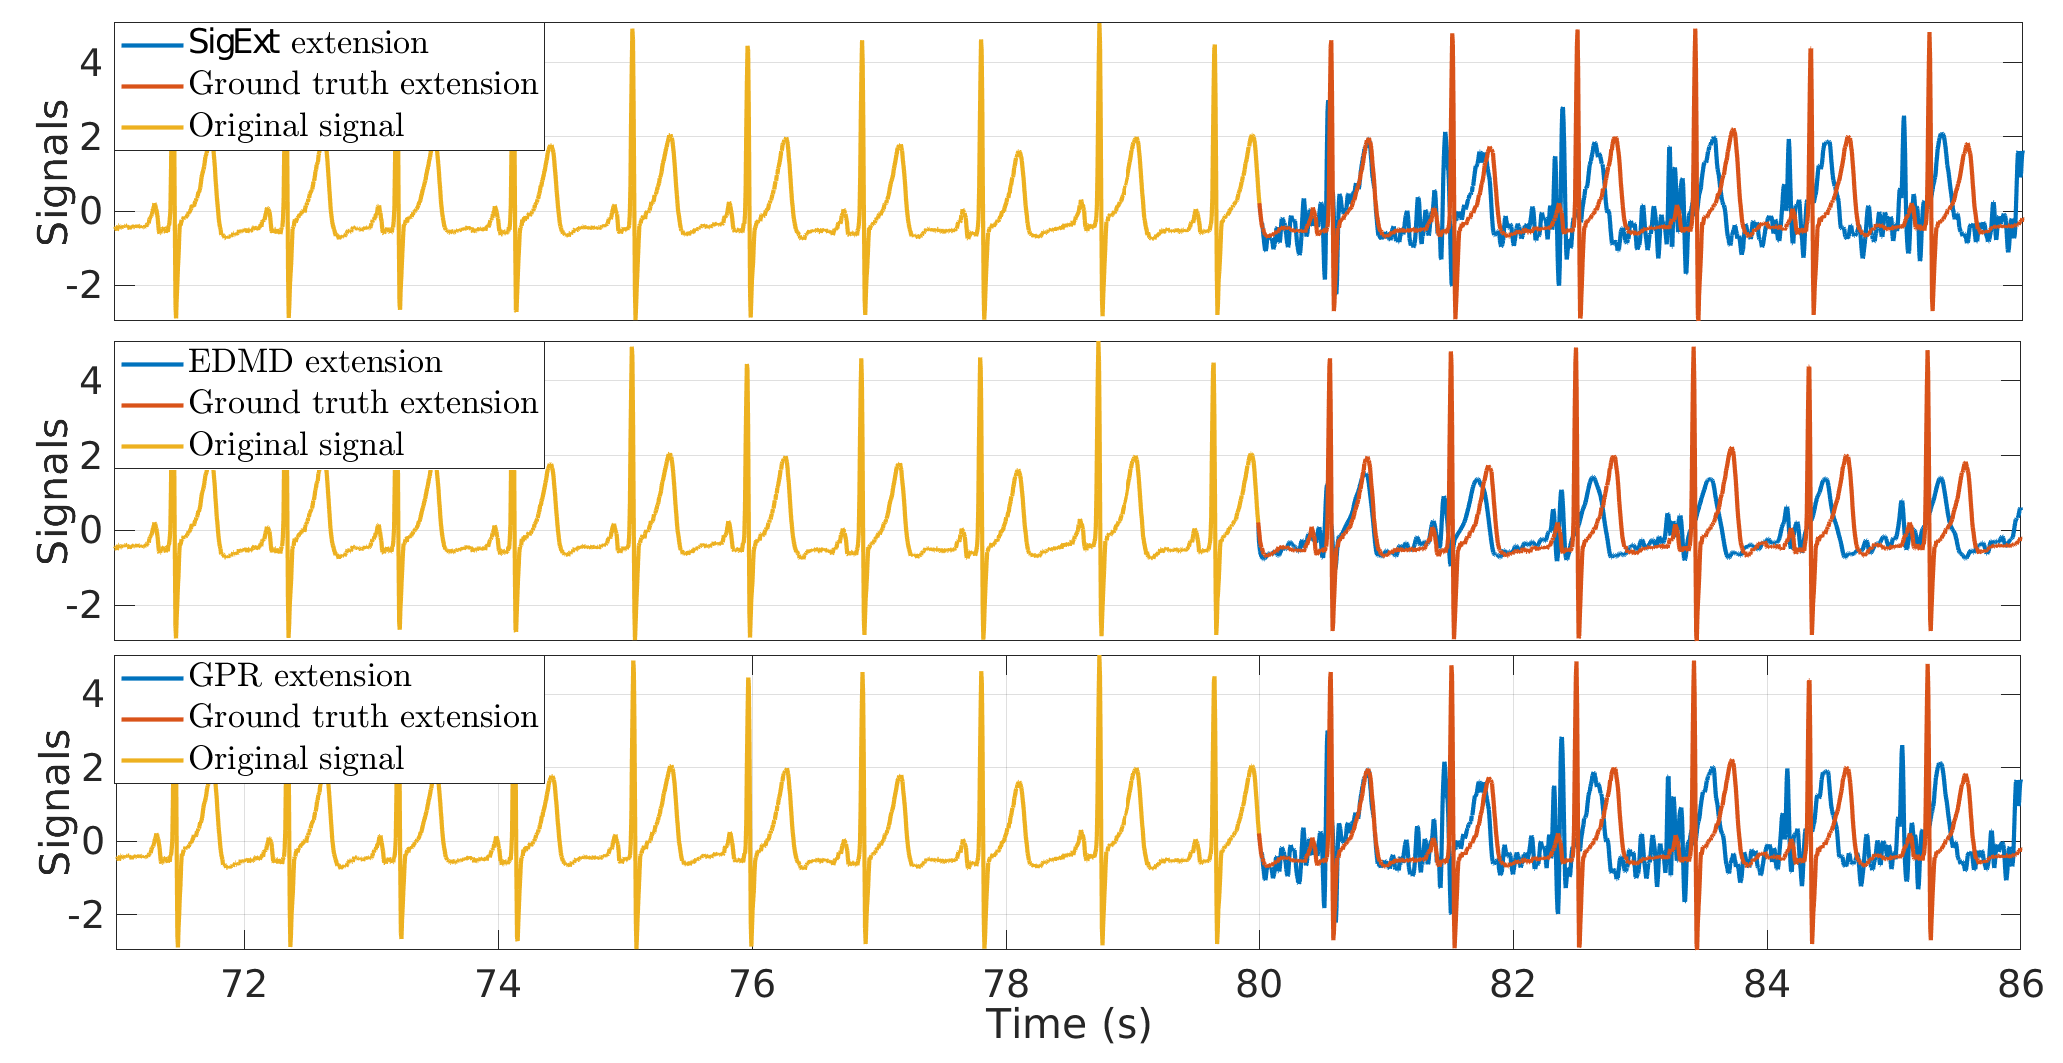
\includegraphics[width=\textwidth]{ECGforecast.eps}
\caption{Extended ECG (blue) obtained by the {\sf SigExt} forecasting (top), the EDMD forecasting (middle), and the GPR forecasting (bottom), superimposed with the ground truth signal (red).}
\label{fig:ecg}
\end{figure}

Table~\ref{tab:otd.ecg} contains the performance index $D$ of the boundary-free TF representations, averaged over the $N$ subsignals, according to the extension method. As a result of the fair quality of the forecasts, the reduction of boundary effects is less significant than for PPG signal. Nevertheles, the results show that {\sf BoundEffRed} has the same efficiency when the {\sf SigExt} extension, the EDMD extension or the GPR extension is chosen. This justifies the choice of {\sf SigExt} for real-time implementation.

\begin{table}
\centering
\caption{ECG: Performance of the Boundary-Free TF Representations According to the Extension Method}
\begin{tabular}{|c||c|c|c|c|}
  \hline
   \multirow{2}{40pt}{\centering Extension method} & \multicolumn{4}{c|}{Averaged performance index $D$} \\
   \cline{2-5}
      & STFT & SST & ConceFT & RS\\
   \hhline{|=#=|=|=|=|}
   {\sf SigExt} & $0.713$ & $0.700$ & $0.753$ & $0.761$ \\
   \hline
   Symmetric & $1.395$ & $1.402$ & $1.416$ & $0.976$ \\
   \hline
   EDMD & $0.856$ & $0.792$ & $0.559$ & $0.688$ \\
   \hline
   GPR & $0.723$ & $0.734$ & $0.734$ & $0.761$ \\
   \hline
\end{tabular}
\label{tab:otd.ecg}
\end{table}

\end{document}